\documentclass[12pt]{article}

\usepackage[utf8]{inputenc}
\usepackage{amsmath}
\usepackage{fancyhdr}
\usepackage{graphicx}
\usepackage{vmargin}
\usepackage{chemfig}
\usepackage{tikz}
\usepackage{pgfplots}

%%%%%%%%%%%%%%%%%%%%%%%%%%%%%%%%%%%%%%%%%%%%%%%%%%%%%%%%%%%%%%%%%%%%%%%%%%

\setmarginsrb{3 cm}{2.5 cm}{3 cm}{2.5 cm}{1 cm}{1.5 cm}{1 cm}{1.5 cm}
\pagestyle{fancy}
\fancyhf{}
\rhead{2-5-2018}
\chead{Matematik aflevering 13}
\lhead{Jeppe Møldrup}
\rfoot{side \thepage}

%%%%%%%%%%%%%%%%%%%%%%%%%%%%%%%%%%%%%%%%%%%%%%%%%%%%%%%%%%%%%%%%%%%%%%%%%%

\begin{document}

\Large{\textbf{Matematik aflevering 13}}
\normalsize

\section*{Opgave 3.}
  Jeg starter med bare at integrere min funktion $f(x)=4x^3-8x$
  $$\int 4x^3-8x \ dx = x^4-\frac{8}{2}x^2+k$$
  Så indsætter jeg mit punkt ind i funktionen og isolerer k
  $$5=1^4-4 \cdot 1^2+k \leftrightarrow k=5-(1-4)=8$$
  Så værdien for k hvis grafen skal skære i punktet $P(1,5)$ vil være $8$

\section*{Opgave 5.}
  Tegn en mulig graf der opfylder at
  $$f(0)=5 \ f(10)=-1$$
  Og at fortegn og nulpunkter for $f'$ er som angivet på tallinien
  \begin{center}
    \begin{tabular}{c c c c c c}
      x && 3 && 7 &\\
      \hline
      $f'(x)$ & - & 0 & + & 0 & -
    \end{tabular}
  \end{center}
  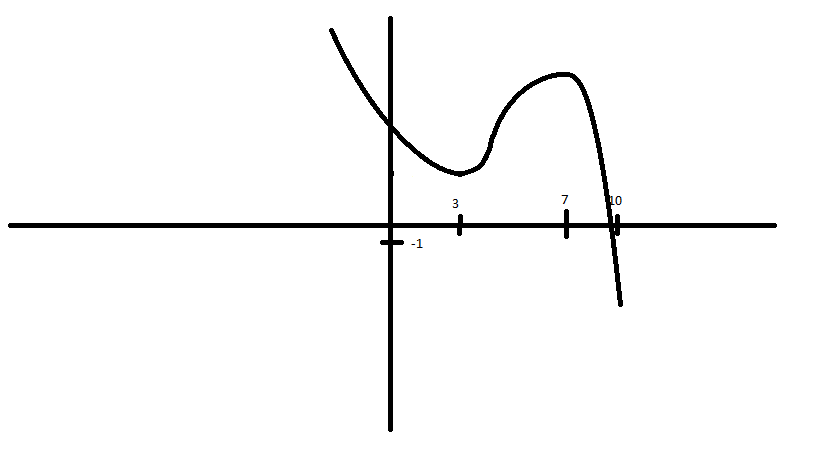
\includegraphics[width=\textwidth]{Graf1mat13.png}

\section*{Opgave 6.}
  Jeg benytter TI-nspire til at finde den kummulerede frekvens for alderen
  derefter aflæser jeg x-værdierne til y-værdierne 25, 50 og 75 for at finde
  kvartilsættet\\
  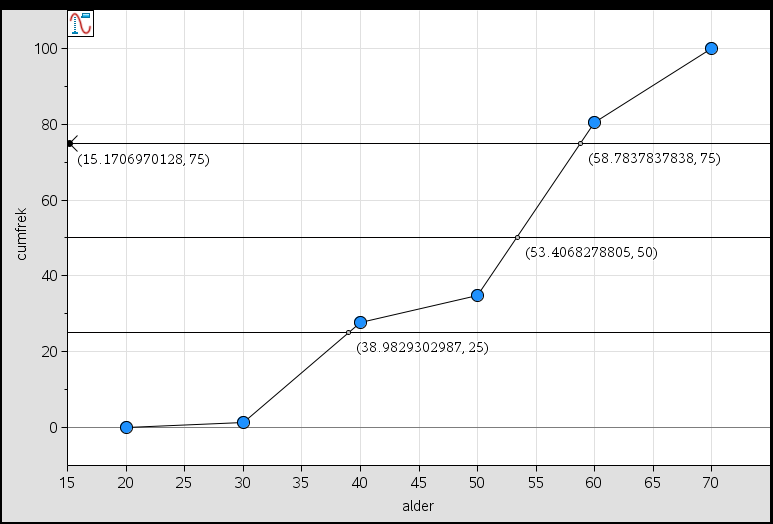
\includegraphics[width=\textwidth]{sumkurve.png}
  kvartilsættet er aflæst til\\
  $$Q_1=39.0 \ Median=53.4 \ Q_3=58.8$$

\section*{Opgave 12.}
  En funktion $f$ er givet ved
  $$f(x)=x^2 ln(x)-3x-1, \ x>0$$
  \begin{enumerate}
    \item[a.] Jeg stater med at differentiere funktionen f
    $$f'(x)=2x \cdot ln(x)-x-3$$
    Så finder jeg den tilhørende y-værdi til x-værdien 1
    $$f'(1)=-2$$
    Så nu har jeg hældningen af grafen, og da jeg ved at grafen går gennem
    punktet $P(1, f(1))$ kan jeg indsætte værdierne i skabelonen
    $$y=a \cdot (x-x_{0}) + y_{0}$$
    $$y=-2(x-1)+(-4)=-2x-2$$
    Så funktionen for tangenten til punktet $P(1, f(1))$ ville være $y=-2x-2$

    \item[b.] Jeg finder samtlige mulige ekstremaer ved at finde alle x-værdier hvor $f'(x)=0$
    $$solve(f'(x)=0,x) \ x=1.57$$
    Så kigger jeg på områderne før og efter mit mulige ekstrema for at se om området er voksende eller aftagende
    $$f'(1)=-2 \ f'(2)=1.77$$
    Nu kan jeg tegne monotonilinien
    \begin{center}
      \begin{tabular}{c c c c}
        x && $1.57$ &\\
        \hline
        $f'(x)$ & - & 0 & +\\
        $f(x)$ & $\searrow$ & $globalt \ min$ & $\nearrow$
      \end{tabular}
    \end{center}
    Så grafen aftager indtil den rammer x-værdien 1.57 og så vokser den derfra
  \end{enumerate}

\section*{Opgave 13.}
  To funktioner $f$ og $g$ er bestemt ved
  $$f(x)=\frac{1}{64}x^2 \ og \ g(x)=\sqrt{x}$$
  Graferne for funktionerne f og g afgrænser i første kvadrant en punktmængde M, der har
  et areal.\\
  Jeg starter med at finde de to x-værdier der argrænser punktmængden dvs. hvor de to grafer skærer hinanden
  $$solve(f(x)=g(x),x) \rightarrow x=0 \vee 16$$
  Så integrere jeg de to funktioner i det inderval og finder den numeriske værdi af differencen
  $$|\int_{0}^{16} (\frac{1}{64}x^2)-(\sqrt{x}) \ dx|=21. \overline{3}$$
  Så arealet af punktmassem m er $21. \overline{3}$

\section*{Opgave 15.}
  I en have skal anlægges et blomsterbed, der har form som et cirkeludsnit
  Det oplyses, at arealet af blomsterbedet som funktion af vinklen v (målt i radianer) er
  $$A(v)=\frac{200v}{(v+2)^2}$$
  Jeg starter med at finde samtlige mulige ekstremaer dvs. hvor hældningen til grafen er 0
  $$solve(A'(v)=0,v) \rightarrow v=2$$
  Det er så mit globale maximum, da det er det eneste ekstrema.
  dvs. at i punktet med x-værdien 2 vil arealet være størst

\section*{Opgave 16.}
  En funktion $f$ er bestemt ved $f(x)=5-x^4$\\
  Et rektangel med højden h, hvor $0 < h < 5$, er placeret som vist på figuren.
  \begin{enumerate}
    \item[a.] For at finde bredden indsætter jeg højden ind på y's plads i forskriften og isolerer 2x
    $$h=5-x^4 \leftrightarrow 2\sqrt[4]{h+5}=2x$$
    2x vil så være bredden, grunden til at det er 2x er fordi at x vil være fra origo eller fra midten af rektanglen og derfor ville kun være
    halvdelen af bredden.\\
    For at finde arealet tager jeg min funktion for bredden og ganger med højden
    $$T=2h\sqrt[4]{h+5}$$
  \end{enumerate}

\section*{Opgave 17.}
Der løber vand fra en vandhane ned i et badekar med en hastighed på 0.4 L/s.
Bundproppen i badekaret er lidt utæt, så vandet løber samtidigt ud af badekarret med en
hastighed, der er proportional med vandmængden i badekarret (målt i L). Det oplyses, at
proportionalitetskonstanten er $0.001 \ s^{/1}$.
\begin{enumerate}
  \item[a.] Jeg starter med at finde ændringen fra vandhanen
  $$\int 0.4 \ L/s \ dx$$
  derefter ændringen fra den utætte bundprop
  $$\int -0.001 \ s^{-1} \cdot x \ dx$$
  Så lægger jeg dem sammen
  $$\int 0.4 \ L/s+(-0.001 \ s^{-1} \cdot x)\ dx = 0.4 \cdot x-5 \cdot 10^{-4} \cdot x^{2}$$
  Så ændringen af vandet i badekarret som funktion af tid ville være\\ $L(t)=0.4 \cdot t-5 \cdot 10^{-4}\cdot t^{2}$
\end{enumerate}

\end{document}
